% Template LaTeX document for CSSR4Africa Deliverables
% Adapted from documents prepared by EPFL for the RobotCub project
% and subsequently by the University of Skövde for the DREAM project
%
% DV 28/06/2023
\PassOptionsToPackage{table,dvipsnames,svgnames,x11names}{xcolor}
\documentclass{CSSRforAfrica}

\usepackage[hidelinks,colorlinks=false]{hyperref}
\usepackage{hyperref}
\hypersetup{
    colorlinks=true,
    linkcolor=black,
    filecolor=blue,      
    urlcolor=blue,
    }

\usepackage[titletoc,title]{appendix}
\usepackage{latexsym}
\usepackage{graphicx}
\usepackage{lscape}
\usepackage{pdflscape}
\usepackage{amsmath}
%\usepackage[table,dvipsnames,svgnames,x11names]{xcolor}
\usepackage{listings}
\usepackage{tabularx}
\usepackage{forest}
\usepackage{dirtree}
\usepackage{float}
\usepackage{siunitx}
\usepackage{tikz}
\usetikzlibrary{shapes.geometric, arrows, positioning, calc}
\usepackage{algorithm}
\usepackage{algpseudocode}
\usepackage{url}



\lstset{upquote=true}
\renewcommand{\DTstyle}{\footnotesize\sffamily}
%%% for listing ;
% \captionsetup[figure]{format=hang}
\definecolor{codegreen}{rgb}{0,0.6,0}
\definecolor{greenyellow}{rgb}{0.8, 0.7, 0.10}
\definecolor{backcolour}{rgb}{0.95,0.95,0.95} 

\lstdefinestyle{withoutNumbering}{
    backgroundcolor=\color{backcolour},   
    commentstyle=\color{codegreen},
    keywordstyle=\color{magenta},
    stringstyle=\color{codepurple},
    basicstyle=\ttfamily\small,
    breakatwhitespace=false,         
    breaklines=true,                 
    captionpos=b,                    
    keepspaces=true,                 
    showspaces=false,                
    showstringspaces=false,
    showtabs=false,                  
    tabsize=2
}
%%%%%%%%%%%%%%%%%%%%%%%%%%%%%%%%%%%%%%%%%%%%%%%%%%%
% the following is added for the note box
\usepackage[most]{tcolorbox}
\newtcolorbox{notebox}[1][]{
  colback=yellow!10!white,
  colframe=black!70!white,
  fonttitle=\bfseries,
  title=NOTE,
  #1
}

\newcommand{\blank}{~\\}
\newcommand{\checkbox}{{~~~~~~~\leavevmode \put(-7,-1.5){  \huge $\Box$  }}}

\begin{document}
\input{epsf}

%%
%% SHOULD NOT NEED TO BE CHANGED BEFORE THIS POINT
%% ------------------------------------------------
%%

\deliverable{D5.5.4}            
\title{D5.5.4 Robot Navigation}   

\leadpartner{Carnegie Mellon University Africa}  
\partner{Carnegie Mellon University Africa}  

\revision{1.2}                         
\deliverabledate{26/02/2025}  
\submissiondate{26/02/2025} 
\revisiondate{07/08/2025}  
\disseminationlevel{PU}
\responsible{Birhanu Shimelis Girma} 


\maketitle

\section*{Executive Summary}
%===============================================================
\label{executive_summary}

Deliverable D5.5.4 focuses on developing a software module for Robot Navigation, enabling the Pepper robot to autonomously traverse its environment while considering both static and dynamic obstacles. This module integrates path planning algorithms, including Breadth-First Search (BFS), Dijkstra, and A*. Navigation is executed by identifying waypoints along the planned path and controlling the robot's locomotion from waypoint to waypoint.

\noindent A key feature of this module is the incorporation of culturally sensitive proxemics, derived from the knowledge base created in \href{https://cssr4africa.github.io/deliverables/CSSR4Africa_Deliverable_D1.2.pdf}{Deliverable D1.2} Rwandan Cultural Knowledge. This functionality ensures that the robot maintains appropriate social distances when navigating around humans, enhancing its adaptability and acceptance in human-centered environments.

\noindent The deliverable outlines a software development process that includes requirements definition, module specification, implementation, implementation, and unit testing. These phases are comprehensively documented, adhering to the methodologies established in \href{https://cssr4africa.github.io/deliverables/CSSR4Africa_Deliverable_D3.2.pdf}{Deliverable D3.2}. The navigation module integrates with the robot localization system developed in \href{https://cssr4africa.github.io/deliverables/CSSR4Africa_Deliverable_D4.2.4.pdf}{Deliverable D4.2.4}, ensuring path execution within the robot's environment.

\noindent This integration is critical for navigation, as the robot continuously updates its pose with real-time data from the robotLocalization node. The requirement definition specifies input parameters  control data, and output velocities, ensuring compatibility with the physical robot. All coding activities adhere to the software engineering standards to produce maintainable and reliable code.

\noindent The deliverable concludes with unit testing. The test evaluates that the developed module meets its objectives and delivers reliable navigation performance for the Pepper robot.


\newpage
\pagebreak
\tableofcontents
\newpage

\section{Introduction}
%===============================================================
This document describes the development and implementation of the robotNavigation ROS node, a component enabling the Pepper robot to navigate in the environment while considering both static and dynamic obstacles. This node is designed to compute optimal paths, avoid obstacles, and execute smooth locomotion towards the goals, ensuring safe and efficient navigation. \\

\noindent As part of Task 5.5.4, the robotNavigation node integrates fundamental path planning and localization techniques, leveraging algorithms such as Breadth-First Search (BFS), Dijkstra’s Algorithm, and A* for trajectory computation. A key feature of this node is its adherence to culturally sensitive proxemics (social distance) , derived from the Rwandan Cultural Knowledge Base (as outlined in \href{https://cssr4africa.github.io/deliverables/CSSR4Africa_Deliverable_D1.2.pdf}{Deliverable D1.2}). This ensures that the robot maintains appropriate social distances when interacting with humans, improving its usability in real-world settings. The navigation system operates in physical environment.\\

\noindent This report provides a comprehensive overview of the robotNavigation node, covering node specifications, implementation details, interface design, executing the node and unit testing. The subsequent sections will elaborate on the key functional components of the node, including path planning, and waypoint-based locomotion ensuring clarity in system design and execution.

\newpage

\section{Requirements Definition}
%===============================================================
The robot navigation node provides the Pepper robot with the ability to navigate autonomously through an environment containing static inanimate obstacles and dynamic obstacles such as humans. This deliverable ensures that the node meets user expectations, enabling the robot to compute the shortest path to a target destination and safely move from waypoint to waypoint. The navigation system operates in various scenarios of physical environment. \\

\noindent The node computes the shortest path from the robot's current position to a specified target position and orientation using Breadth First Search or Dijkstra’s algorithm or the A* algorithm. The computed path should include waypoints, which are identified using either equidistant waypoint selection or high path curvature waypoint selection techniques. These methods ensure smooth and efficient navigation along the planned path while considering the robot’s physical capabilities and the complexity of the environment.\\

\noindent The node also requires obstacle avoidance mechanisms. It must augment a pre-defined metric workspace map with additional obstacles, including human obstacles detected in the robot's field of view. The size and extent of these human obstacles must adhere to culturally sensitive proxemics, as defined in \href{https://cssr4africa.github.io/deliverables/CSSR4Africa_Deliverable_D1.2.pdf}{Deliverable D1.2} African Modes of Social Interaction. This ensures that the robot respects personal space and cultural norms during navigation.


\noindent The navigation node is designed to integrate with other systems. It acquires the robot’s current pose from the robotLocalization node, and uses the workspace map generated in \href{https://cssr4africa.github.io/deliverables/CSSR4Africa_Deliverable_D5.5.3.pdf}{Deliverable D5.5.3}. The node then publishes the planned path and velocity commands to the \texttt{/cmd\_vel} topic, enabling the robot’s locomotion.

\noindent The node operates in two modes, normal mode and verbose mode. In normal mode, it executes navigation without additional logging or visualization. In verbose mode, it logs data published to topics and displays diagnostic information, such as the configuration space map and planned path, in an OpenCV window. This dual-mode functionality allows for detailed debugging and analysis during development and testing.

\noindent To initiate navigation, the node accepts a goal pose specified by the coordinates $x, y$ and an orientation $\theta$ in the workspace frame of reference. Once the goal is received, the node calculates the required path and outputs a sequence of forward and angular velocities, which are published to the \texttt{/cmd\_vel} topic. Additionally, the configuration space map and the planned path are rendered graphically for analysis.

\noindent Operationally, the node is compatible with both the physical Pepper robot and a simulated environment using the Pepper simulator. It reads platform-specific parameters, such as sensor and actuator topics, from a configuration file named \verb|robotNavigationConfiguration.ini|. This ensures that the node can be easily adapted to different platforms without altering its core logic.

\noindent From a non-functional perspective, the node is designed to compute the shortest path to ensure real-time navigation. The robot must reach its target position within a predefined tolerance $(\pm \SI{0.1}{\meter} \text{ for position and} \pm \SI{5}{\degree}\text{ for orientation})$. The node must also demonstrate a high success rate (e.g., $\geq{95}$\%) in avoiding obstacles during navigation. To ensure maintainability, the code adheres to the software engineering standards outlined in \href{https://cssr4africa.github.io/deliverables/CSSR4Africa_Deliverable_D3.2.pdf}{Deliverable D3.2}, and internal documentation clearly describes the node’s functionalities, parameters, and interfaces.

\noindent In its intended use, the node must navigate static environments using a pre-defined workspace map. The robot must also dynamically adjust its behavior when humans or other obstacles enter its path, ensuring safe and efficient navigation.


\newpage

\section{Module Specification}
%===============================================================
The Robot Navigation node is designed to facilitate autonomous navigation for the Pepper robot by computing paths, avoiding obstacles, and ensuring cultural proxemics are respected. This node integrates path planning algorithms such as Breadth-First Search (BFS), Dijkstra, and A* to determine the optimal trajectory between waypoints while maintaining real-time awareness of the environment.

\subsection*{Path Planning Algorithms}
The robotNavigation node implements three distinct path planning algorithms, each with specific characteristics suitable for different navigation scenarios. The selection of the appropriate algorithm is determined by the \texttt{pathPlanning} parameter in the \texttt{robotNavigationConfiguration.ini} file. \\

\noindent \textbf{Breadth-First Search (BFS):} A fundamental graph traversal algorithm that explores all neighbor nodes at the current depth before moving to nodes at the next depth level \cite{cormen2009introduction}. 
\begin{figure}[H]
	\centering
	\begin{minipage}{0.8\textwidth}
		\begin{algorithm}[H]
			\caption{Breadth-First Search (BFS)}
			\begin{algorithmic}[1]
				\Function{BFS}{$start, goal, graph$}
				\State Initialize empty queue $Q$
				\State Initialize $visited$ array with all nodes marked as $false$
				\State Initialize $predecessor$ array with all nodes set to $-1$
				
				\State Mark $start$ as visited
				\State Enqueue $start$ to $Q$
				
				\While{$Q$ is not empty}
				\State $current \gets$ Dequeue from $Q$
				
				\If{$current$ equals $goal$}
				\State Reconstruct path from $predecessor$ and return
				\EndIf
				
				\For{each $neighbor$ of $current$ in $graph$}
				\If{$neighbor$ not visited}
				\State Mark $neighbor$ as visited
				\State Set $predecessor[neighbor] \gets current$
				\State Enqueue $neighbor$ to $Q$
				\EndIf
				\EndFor
				\EndWhile
				
				\State \Return empty path (no path found)
				\EndFunction
			\end{algorithmic}
		\end{algorithm}
	\end{minipage}
	\caption{Pseudocode for the BFS algorithm implementation}
	\label{alg:bfs}
\end{figure}


\noindent BFS uses a queue-based approach with 4-way movement (up, down, left, right) and guarantees finding the shortest path in terms of the number of grid cells traversed. It is preferred in scenarios with uniform cost grids and when computational efficiency is prioritized over path optimality in terms of actual distance. It has simple implementation, guaranteed shortest path in terms of steps (not distance), and no need for heuristic function as shown in figure \ref{alg:bfs}. It is Less efficient in large spaces, doesn't account for diagonal movements or varying costs, and explores nodes in all directions equally.\\

\noindent \textbf{Dijkstra's Algorithm:} A weighted graph search algorithm that finds the shortest path from a starting node to all other nodes in the graph, accounting for varying edge weights \cite{Dijkstra1959}.
\begin{figure}[H]
	\centering
	\begin{minipage}{0.8\textwidth}
		\begin{algorithm}[H]
			\caption{Dijkstra's Algorithm}
			\begin{algorithmic}[1]
				\Function{Dijkstra}{$start, goal, graph$}
				\State Initialize $dist$ array with all nodes set to $INFINITY$
				\State Initialize $predecessor$ array with all nodes set to $-1$
				\State Initialize priority queue $PQ$
				
				\State Set $dist[start] \gets 0$
				\State Insert $(0, start)$ to $PQ$
				
				\While{$PQ$ is not empty}
				\State Extract node with minimum distance as $current$
				
				\If{$current$ equals $goal$}
				\State Reconstruct path from $predecessor$ and return
				\EndIf
				
				\For{each $neighbor$ of $current$ in $graph$}
				\State $new\_dist \gets dist[current] + 1$  // Cost is uniform in our implementation
				\If{$new\_dist < dist[neighbor]$}
				\State $dist[neighbor] \gets new\_dist$
				\State $predecessor[neighbor] \gets current$
				\State Insert $(new\_dist, neighbor)$ to $PQ$
				\EndIf
				\EndFor
				\EndWhile
				
				\State \Return empty path (no path found)
				\EndFunction
			\end{algorithmic}
		\end{algorithm}
	\end{minipage}
	\caption{Pseudocode for the Dijkstra's algorithm implementation}
	\label{alg:dijkstra}
\end{figure}


\noindent Dijkstra uses a priority queue with 8-way movement (including diagonals) and selects the node with the lowest cumulative path cost at each step. It is optimal for navigation in environments with varying traversal costs, such as terrain with different friction coefficients or spaces with different levels of congestion. It guarantees finding the optimal path in terms of cost, and can handle varying edge weights. It is less efficient than informed search algorithms like A* since it explores nodes in all directions equally without using a heuristic as shown in figure \ref{alg:dijkstra}.\\

\noindent \textbf{A* Algorithm:} An informed search algorithm that combines Dijkstra's cost-so-far approach with a heuristic estimate of the cost to the goal, effectively prioritizing paths that seem promising \cite{A*}.
\begin{figure}[H]
	\centering
	\begin{minipage}{0.8\textwidth}
		\begin{algorithm}[H]
			\caption{A* Algorithm}
			\begin{algorithmic}[1]
				\Function{AStar}{$start, goal, graph, cols, heuristic\_type$}
				\State Select heuristic function based on $heuristic\_type$
				\State Initialize $dist$ array with all nodes set to $INFINITY$
				\State Initialize $predecessor$ array with all nodes set to $-1$
				\State Initialize priority queue $PQ$
				
				\State Set $dist[start] \gets 0$
				\State Insert $(0 + heuristic(start, start, goal, cols), start)$ to $PQ$
				
				\While{$PQ$ is not empty}
				\State Extract node with minimum f-value as $current$
				
				\If{$current$ equals $goal$}
				\State Reconstruct path from $predecessor$ and return
				\EndIf
				
				\For{each $neighbor$ of $current$ in $graph$}
				\State $new\_dist \gets dist[current] + 1$  // Cost is uniform in the implementation
				\If{$new\_dist < dist[neighbor]$}
				\State $dist[neighbor] \gets new\_dist$
				\State $predecessor[neighbor] \gets current$
				\State $priority \gets new\_dist + heuristic(current, neighbor, goal, cols)$
				\State Insert $(priority, neighbor)$ to $PQ$
				\EndIf
				\EndFor
				\EndWhile
				
				\State \Return empty path (no path found)
				\EndFunction
			\end{algorithmic}
		\end{algorithm}
	\end{minipage}
	\caption{Pseudocode for the A* algorithm implementation}
	\label{alg:astar}
\end{figure}



\noindent A* uses a priority queue with 8-way movement and employs either Manhattan or Euclidean distance as a heuristic to guide the search. The node allows selection between these heuristics for different navigation scenarios. A* is the default and preferred choice for most navigation scenarios as it provides an optimal balance between computational efficiency and path optimality, especially in complex environments with obstacles. It is more efficient than Dijkstra's algorithm as it uses a heuristic to guide the search toward the goal, guarantees finding the optimal path if the heuristic is admissible, and can handle varying edge weights as shown in figure \ref{alg:astar}. The performance depends on the quality of the heuristic; an inappropriate heuristic can lead to suboptimal paths or increased computational cost.\\


\noindent The system selects the appropriate path planning algorithm based on the \texttt{pathPlanning} parameter specified in the \texttt{robotNavigationConfiguration.ini} file, allowing users to choose between BFS, Dijkstra, or A* algorithms to optimize for different navigation scenarios. This flexibility ensures that the Pepper robot can effectively navigate through various scenarios while respecting both physical constraints and cultural proxemics.


\noindent The navigation process follows a structured approach: First, the node computes the shortest path from the robot’s current position to the specified goal \( (x, y, \theta) \) using a selected algorithm. Once the path is determined, it is discretized into intermediate waypoints to facilitate smooth navigation. The system checks its configuration space to account for static obstacles, ensuring safe movement. Finally, the robot executes the planned trajectory by adjusting its velocity and rotation commands, allowing it to reach the target destination efficiently.\\


\noindent The configuration space map is used to define accessible areas within the robot’s environment. This map is essential for identifying free space, avoiding obstacles, and computing feasible navigation paths. The workspace is represented as an occupancy grid, where white regions indicate navigable areas, and darker regions correspond to obstacles or restricted zones. A sample configuration space map is shown in Figure \ref{fig:config_space_map}.

\begin{figure}[H]
    \centering
    \begin{minipage}{0.49\textwidth}
        \centering
        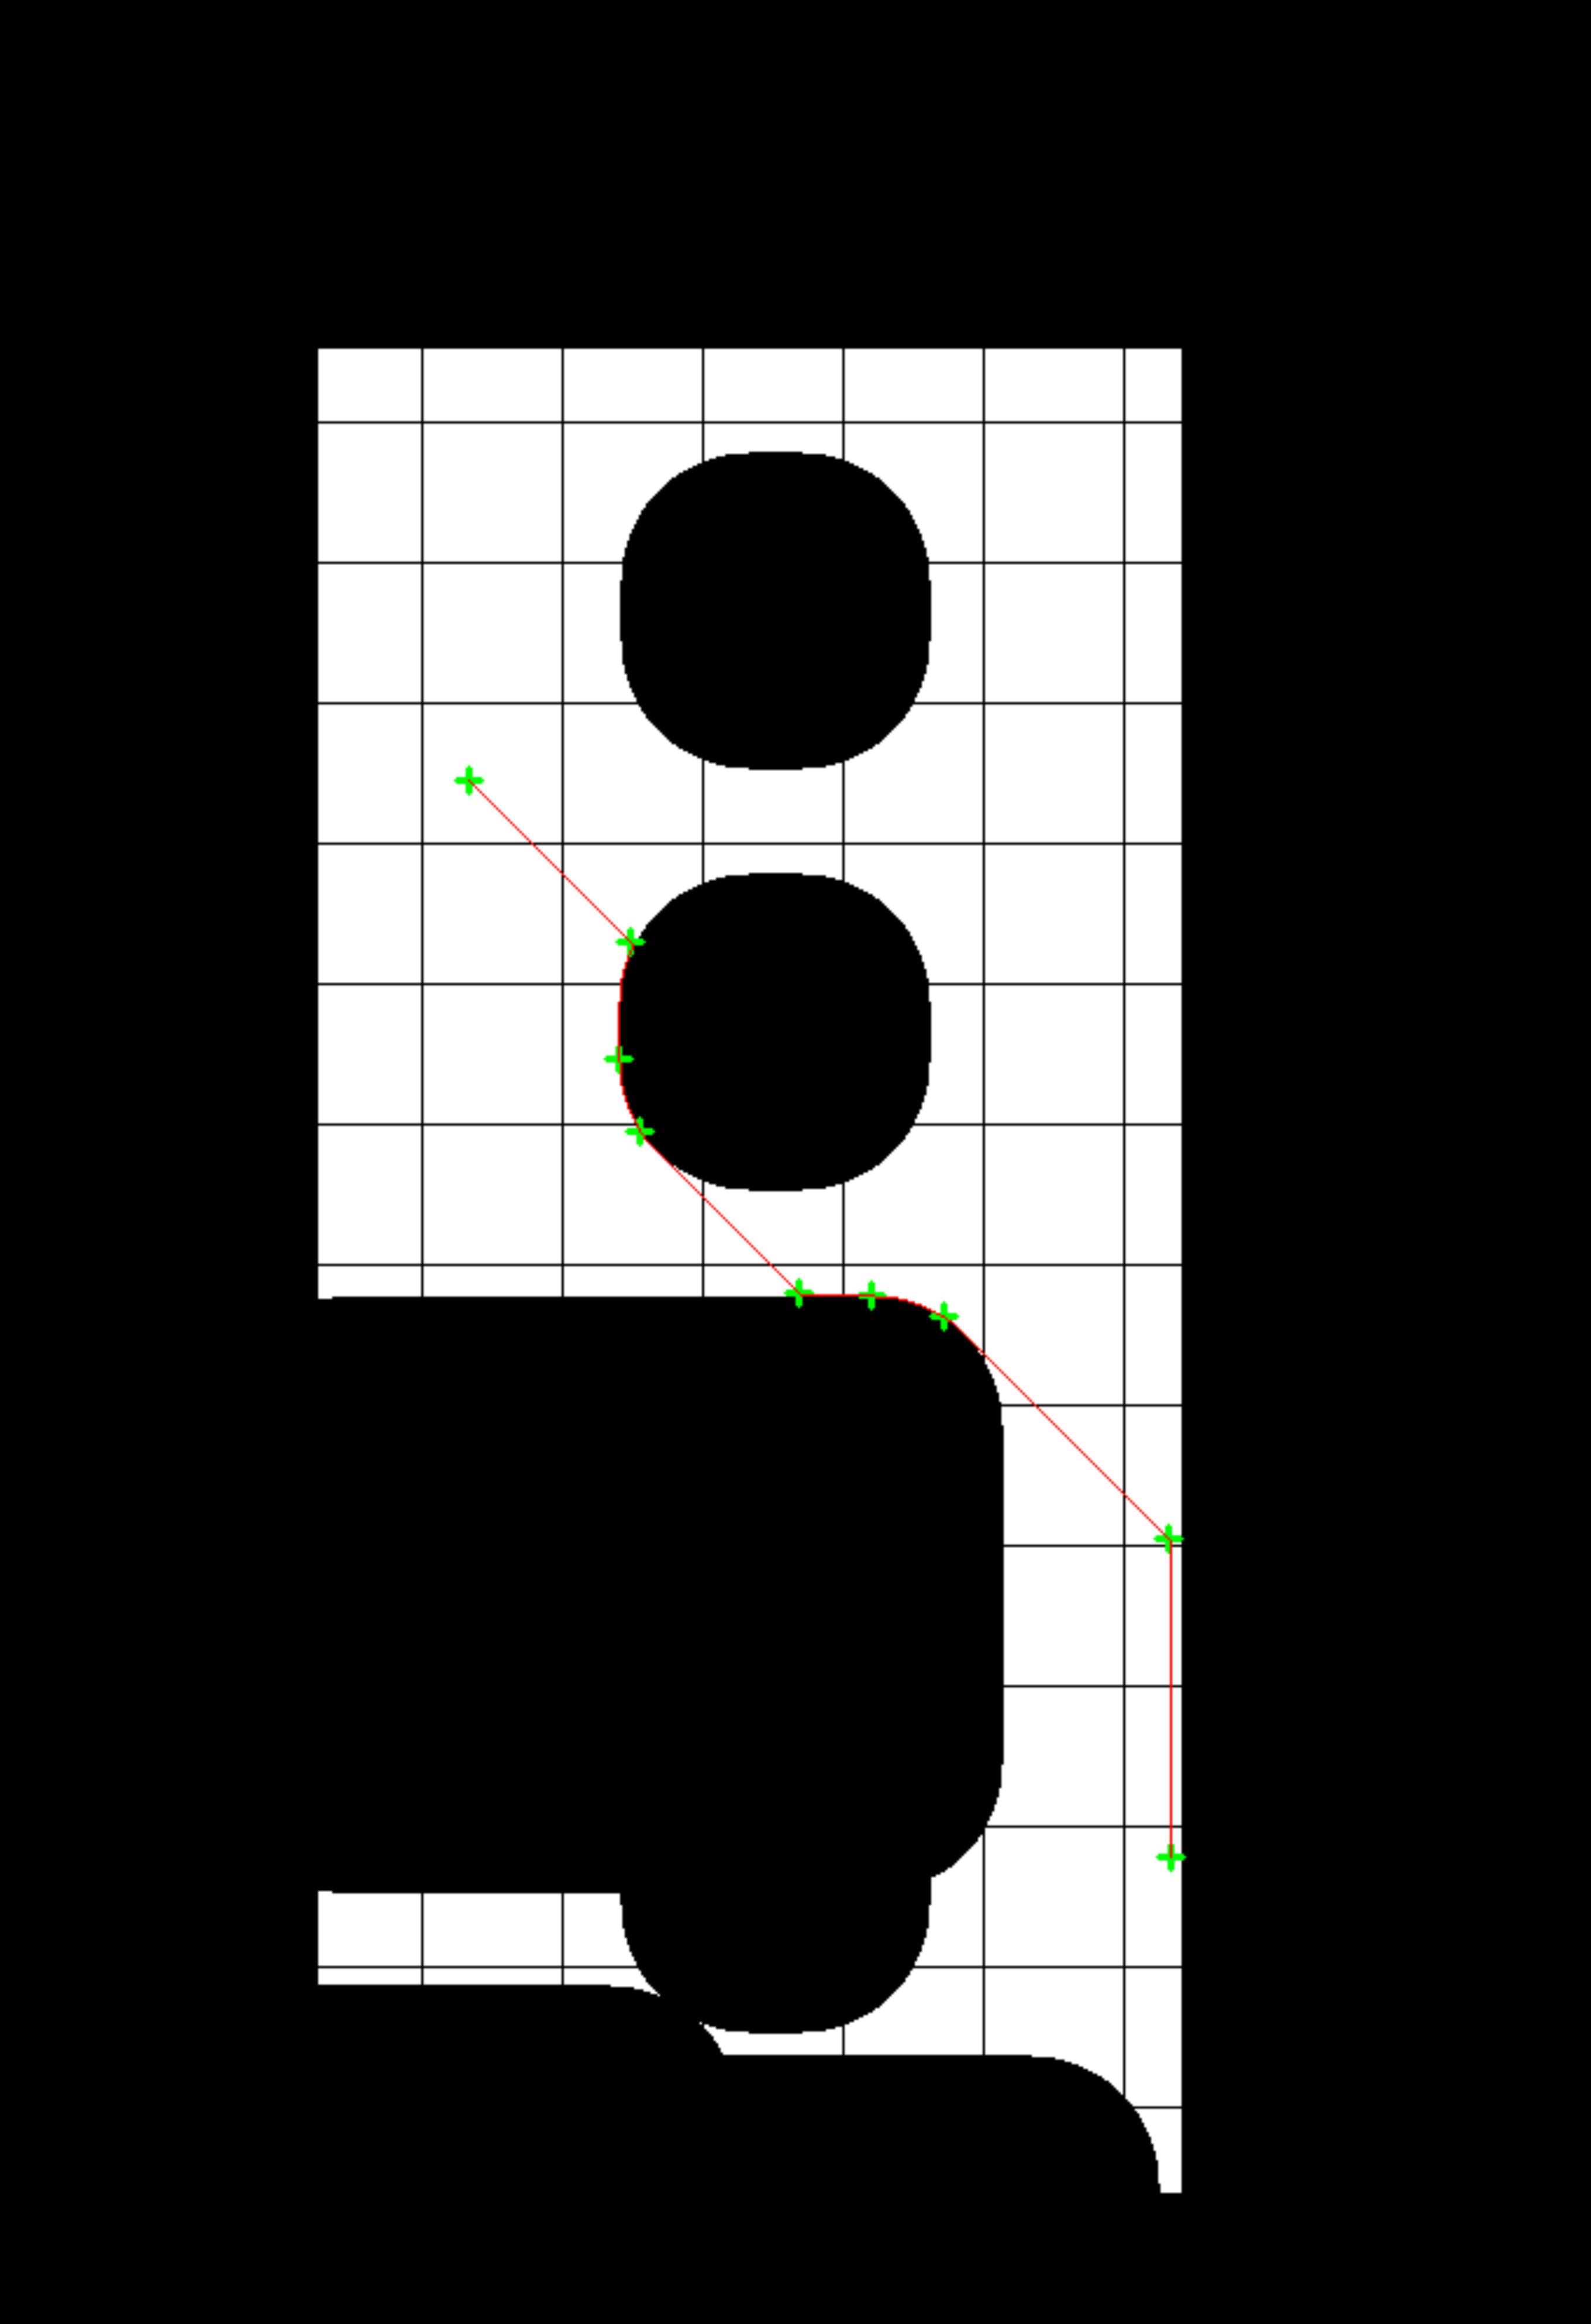
\includegraphics[width=\linewidth]{Images/configMapWaypointsAstar.png}
        \caption{The configuration space map highlights areas that are navigable and restricted, ensuring safe path planning.}
        \label{fig:config_space_map}
    \end{minipage}
    \hfill
    \begin{minipage}{0.49\textwidth}
        \centering
        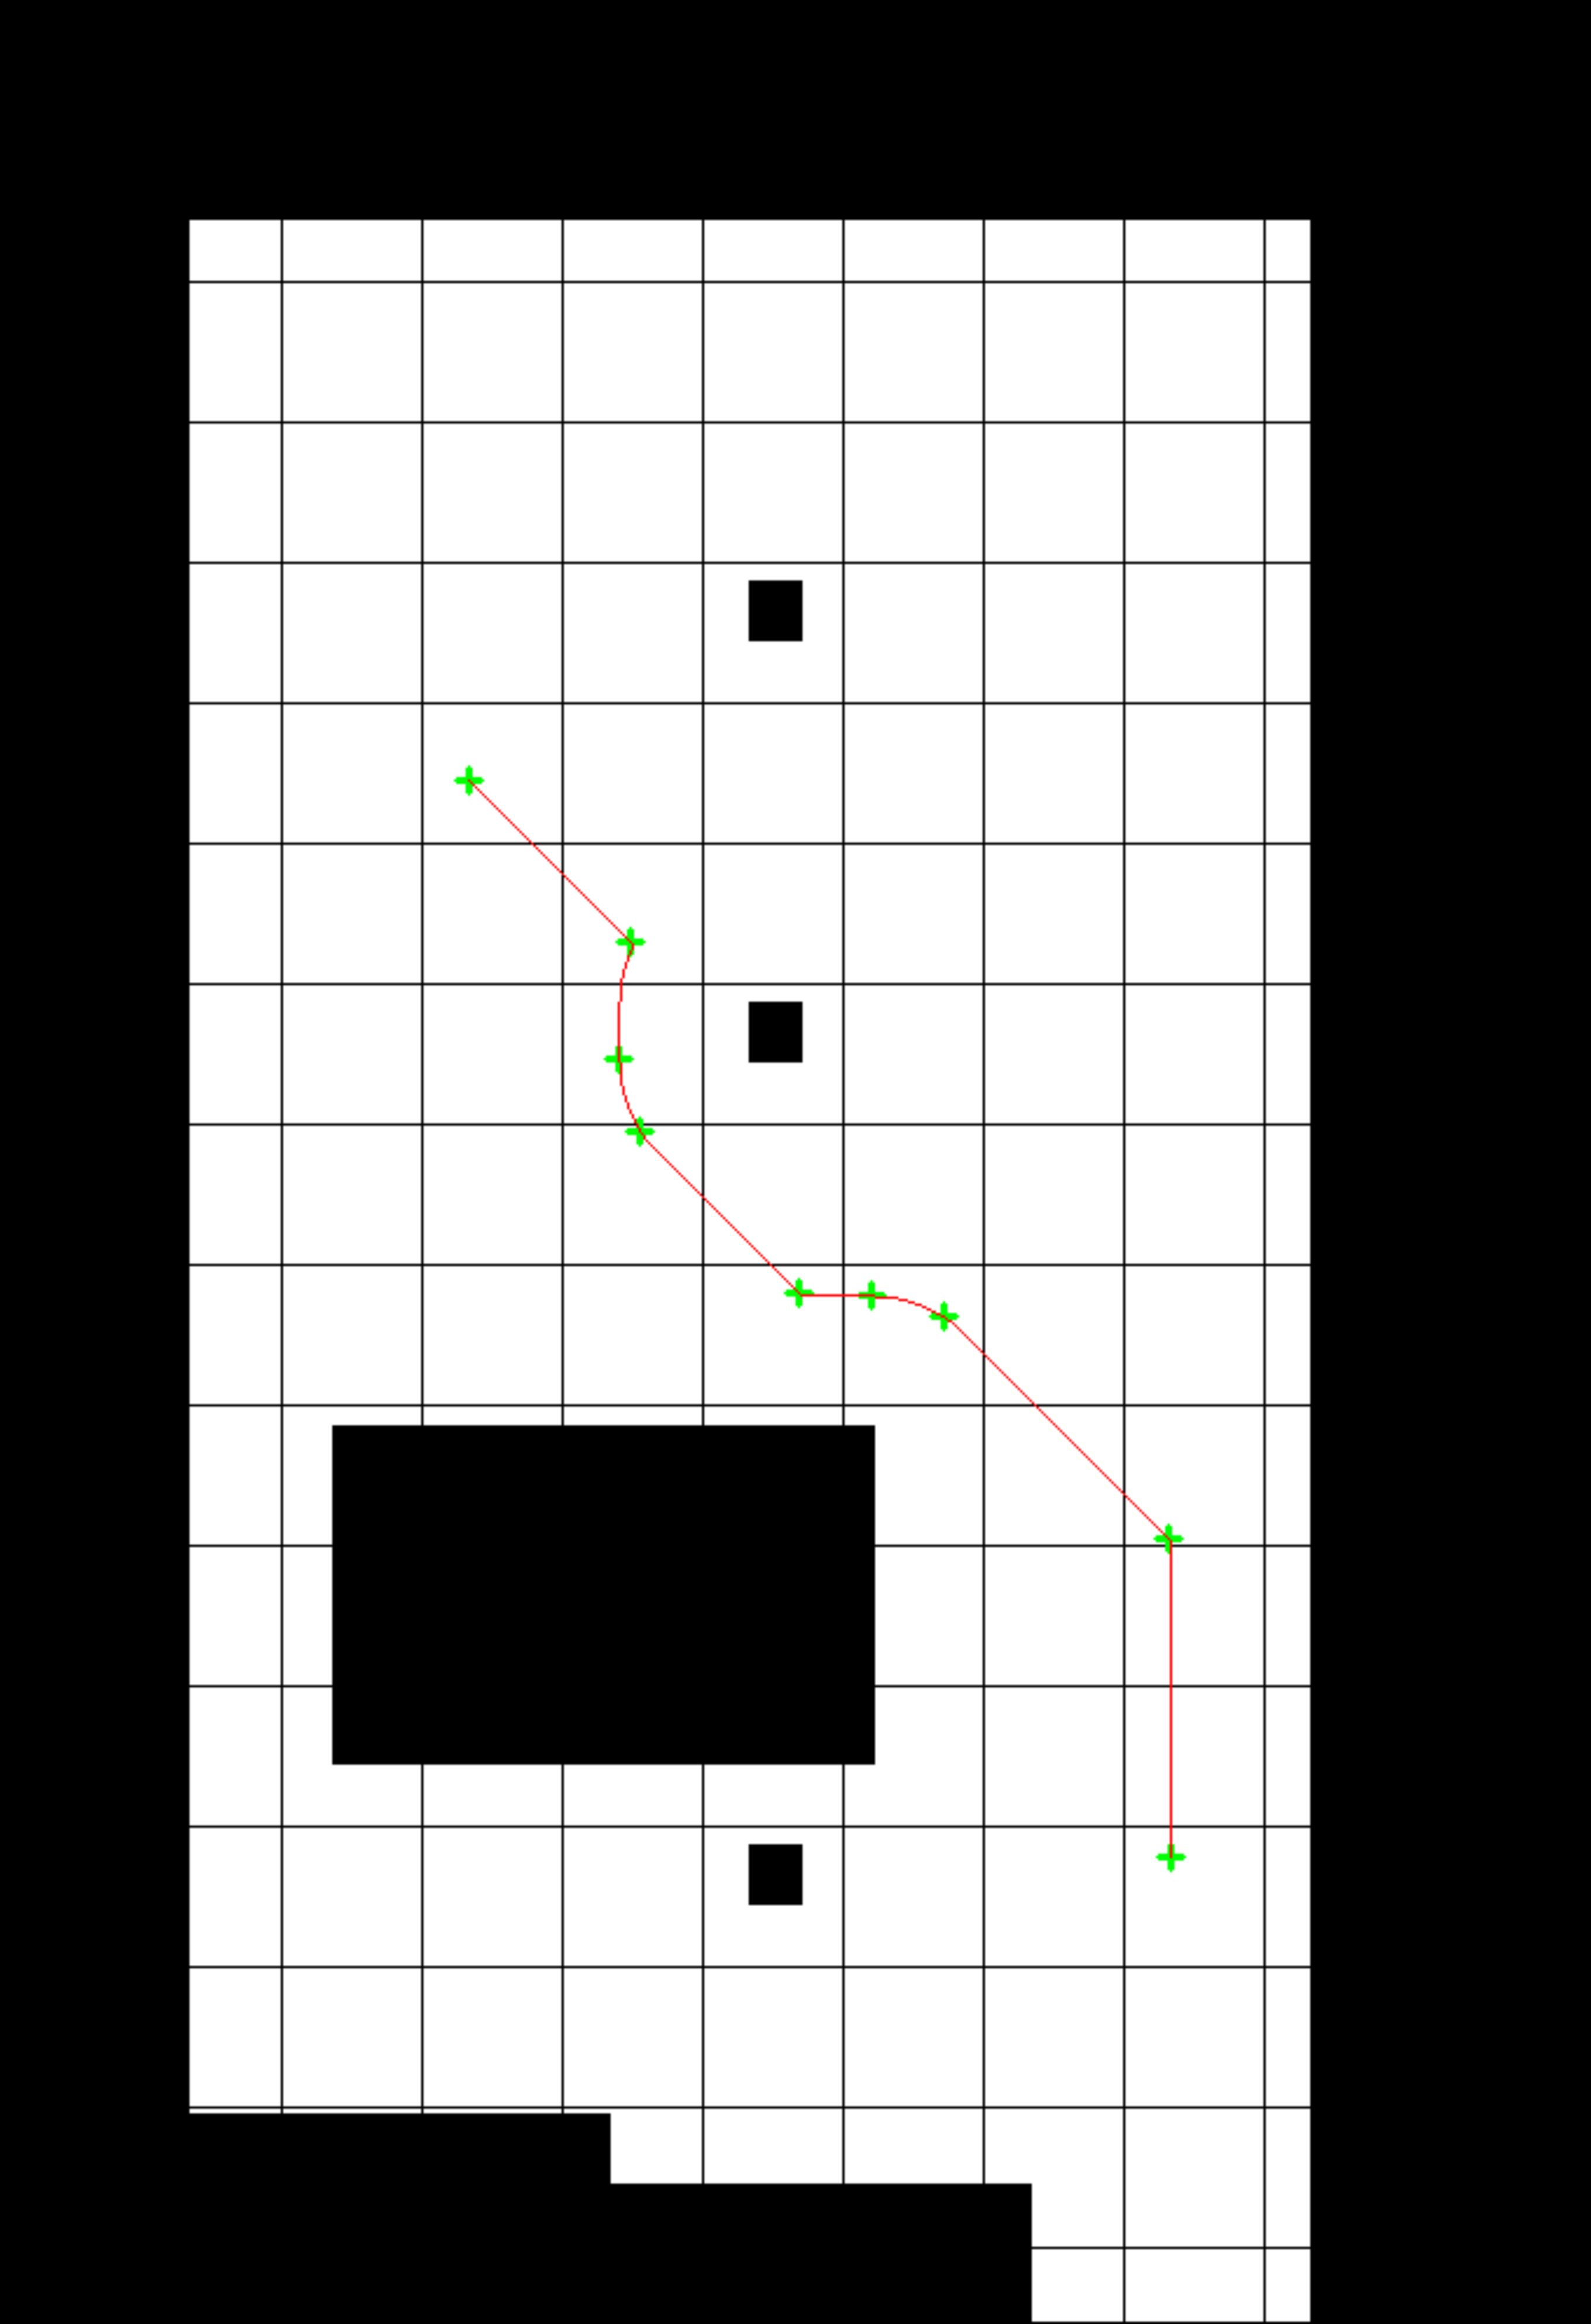
\includegraphics[width=\linewidth]{Images/environmentMapWaypointsAstar.png}
        \caption{Visualization of the A* based waypoint navigation approach. The robot follows the computed waypoints to reach its goal.}
        \label{fig:waypoint_map}
    \end{minipage}
\end{figure}
\noindent To ensure efficient navigation, the node breaks the computed path into discrete waypoints. Each waypoint serves as an intermediate target, guiding the robot smoothly toward its final destination. The robot continuously updates its position and recalculates waypoints when necessary. The map of the waypoints, depicted in Figure \ref{fig:waypoint_map}, illustrates a sample navigation path with sequential waypoints.\\

\noindent The navigation node supports static map navigation, where the robot operates on a predefined map with known obstacles. To execute a navigation task, the node requires an input, which is a goal pose (x, y, $\theta$) provided through a ROS service request. The processing phase involves path computation, waypoint selection, and obstacle detection to ensure safe movement. Finally, the output consists of a sequence of velocity commands that actuate the robot’s wheels, guiding it toward the desired destination.\\

\noindent The robot receives sensory data from the robotLocalization node and adjusts its navigation accordingly. The final execution involves publishing velocity commands to the \texttt{/cmd\_vel} topic, enabling movement toward the desired goal while adhering to safety constraints. A flowchart explaining the robot navigation process is illustrated in figure \ref{fig:navigation_flowchart}.

\begin{figure}[H]
	\centering
	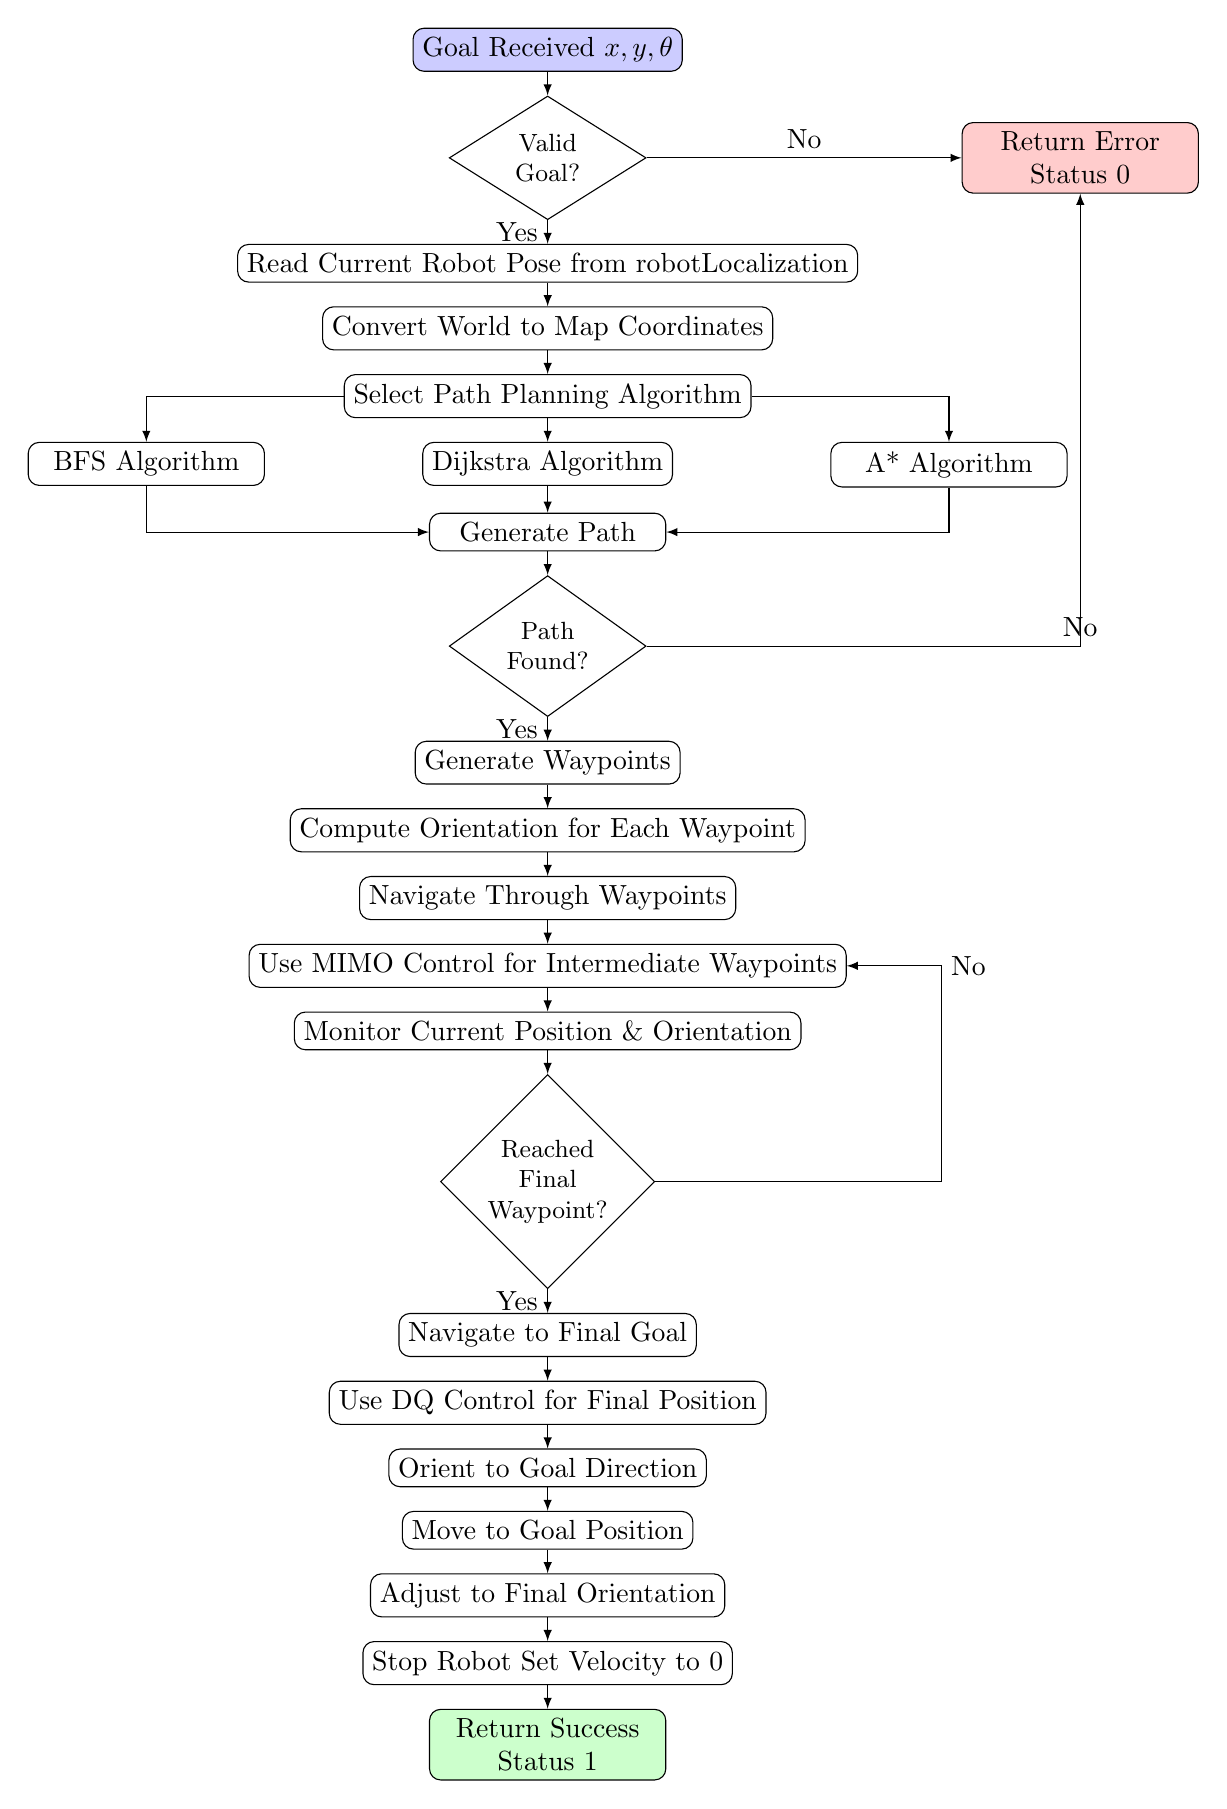
\begin{tikzpicture}[
	node distance = 0.30cm,
	box/.style = {rectangle, draw, text centered, rounded corners, minimum height=0.2cm, minimum width=3cm, align=center},
	decision/.style = {diamond, draw, text centered, minimum height=0.3cm, minimum width=2.5cm, font=\small, align=center, inner sep=1pt},
	line/.style = {draw, -latex}
	]
	
	% Nodes
	\node [box, fill=blue!20] (start) {Goal Received $x, y, \theta$};
	\node [decision, below=of start] (valid) {Valid \\ Goal?};
	\node [box, right=4cm of valid, fill=red!20] (error) {Return Error \\ Status 0};
	\node [box, below=of valid] (pose) {Read Current Robot Pose from robotLocalization};
	\node [box, below=of pose] (convert) {Convert World to Map Coordinates};
	\node [box, below=of convert] (algorithm) {Select Path Planning Algorithm};
	
	% Path planning algorithms
	\node [box, below left=0.3cm and 1cm of algorithm] (bfs) {BFS Algorithm};
	\node [box, below=of algorithm] (dijkstra) {Dijkstra Algorithm};
	\node [box, below right=0.3cm and 1cm of algorithm] (astar) {A* Algorithm};
	
	\node [box, below=1.2cm of algorithm] (path) {Generate Path};
	\node [decision, below=of path] (pathfound) {Path \\ Found?};
	
	% Waypoint generation
	\node [box, below=of pathfound] (waypoints) {Generate Waypoints};
	\node [box, below=of waypoints] (orientation) {Compute Orientation for Each Waypoint};
	
	% Navigation
	\node [box, below=of orientation] (navigate) {Navigate Through Waypoints};
	\node [box, below=of navigate] (mimo) {Use MIMO Control for Intermediate Waypoints};
	\node [box, below=of mimo] (monitor) {Monitor Current Position \& Orientation};
	\node [decision, below=of monitor] (finalwp) {Reached \\ Final \\ Waypoint?};
	
	\node [box, below=of finalwp] (finalnav) {Navigate to Final Goal};
	\node [box, below=of finalnav] (dq) {Use DQ Control for Final Position};
	\node [box, below=of dq] (orient) {Orient to Goal Direction};
	\node [box, below=of orient] (move) {Move to Goal Position};
	\node [box, below=of move] (adjust) {Adjust to Final Orientation};
	
	\node [box, below=of adjust] (stop) {Stop Robot Set Velocity to 0};
	\node [box, below=of stop, fill=green!20] (success) {Return Success \\ Status 1};
	
	% Lines
	\path [line] (start) -- (valid);
	\path [line] (valid) -- node[above] {No} (error);
	\path [line] (valid) -- node[left] {Yes} (pose);
	\path [line] (pose) -- (convert);
	\path [line] (convert) -- (algorithm);
	
	\path [line] (algorithm) -| (bfs);
	\path [line] (algorithm) -- (dijkstra);
	\path [line] (algorithm) -| (astar);
	
	\path [line] (bfs) |- (path);
	\path [line] (dijkstra) -- (path);
	\path [line] (astar) |- (path);
	
	\path [line] (path) -- (pathfound);
	\path [line] (pathfound) -| node[above] {No} (error);
	\path [line] (pathfound) -- node[left] {Yes} (waypoints);
	
	\path [line] (waypoints) -- (orientation);
	\path [line] (orientation) -- (navigate);
	\path [line] (navigate) -- (mimo);
	\path [line] (mimo) -- (monitor);
	\path [line] (monitor) -- (finalwp);
	
	\path [line] (finalwp) -- node[left] {Yes} (finalnav);
	\path [line] (finalwp) -- ++(5,0) |- node[right] {No} (mimo);
	
	\path [line] (finalnav) -- (dq);
	\path [line] (dq) -- (orient);
	\path [line] (orient) -- (move);
	\path [line] (move) -- (adjust);
	\path [line] (adjust) -- (stop);
	\path [line] (stop) -- (success);    
	\end{tikzpicture}
	\caption{Flowchart of the robot navigation process from goal reception to completion}
	\label{fig:navigation_flowchart}
\end{figure}

\newpage

\section{Implementation}
%===============================================================
\subsection{File Organization }
The source code for executing the robot navigation functionality is structured into three primary components: robotNavigationApplication, robotNavigationImplementation, and robotNavigationInterface. The robotNavigationImplementation component encapsulates the core functionality required for robot navigation, including tasks such as path planning, obstacle avoidance, and waypoint management. It supports three algorithms, including BFS, Dijkstra, and A*, and integrates features for cultural proxemics constraints, such as maintaining social distances. This component also processes critical files such as configuration files, map data, and topic definitions to enable smooth navigation. \\

\noindent The robotNavigationApplication serves as the entry point for the navigation node, managing the execution of functions defined in the implementation and interface components. It initializes the ROS node, sets up parameters, and orchestrates the navigation operations. The robotNavigationInterface defines the abstract layer and function declarations that facilitate communication between the application and implementation layers, ensuring modularity and consistency in the codebase. This file structure promotes clean separation of concerns, making the navigation system easier to maintain, extend, and debug while supporting scalable integration with other system components.

\noindent The file structure of the robot navigation node in the \verb|cssr_system| package is organized as follows:

\vspace*{0.5em}
\begin{figure}[H]
	\renewcommand*\DTstyle{\ttfamily}
	\dirtree{%
		.1 cssr\_system.
		.2 robotNavigation.
		.3 config.
		.4 robotNavigationConfiguration.ini.
		.3 data.
		.4 robotTopics.dat.
		.4 environmentMap.png.
		.4 configurationSpaceMap.png.
		.4 prameters230.dat.
		.4 parameters240.dat.
		.4 robotPose.dat.
		.3 include.
		.4 robotNavigation.
		.5 robotNavigationInterface.h.
		.3 msg.
		.4 Goal.msg.
		.3 src.
		.4 robotNavigationApplication.cpp.
		.4 robotNavigationImplementation.cpp.
		.3 srv.
		.4 setGoal.srv.
		.3 README.md.
		.3 CMakeLists.txt.
		.3 package.xml.
	}
	\caption{File structure of the robotNavigation node}
	\label{fig:navigation_file_structure}
\end{figure}

\subsection{Configuration Parameters}
The operation of the \verb|robotNavigation| node is determined by the contents of a configuration file, \verb|robotNavigationConfiguration.ini| that contain a list of key-value pairs as shown below in Table \ref{tab:robotNavigationConfiguration.ini}.

\begin{table}[H]
\centering
\caption{Configuration Parameters for robotNavigation node.}
\label{tab:robotNavigationConfiguration.ini}
\begin{tabularx}{\textwidth}{|l|l|X|}
\hline
\textbf{Key} & \textbf{Values} & \textbf{Effect} \\ \hline
\verb|environmentMap| & \verb|environmentMap.png| & Specifies the workspace map file. \\ \hline
\verb|configurationMap| & \verb|configuratuinSpaceMap.png| & Specifies the configuration space map file. \\ \hline
\verb|pathPlanning| & \verb|BFS, Dijkstra, A*| & Specifies the algorithm for path planning. \\ \hline
\verb|socialDistance| & \verb|true, false| & Enables/disables cultural proxemics constraints. \\ \hline
\verb|robotTopics| & \verb|pepperTopics.dat| & Sensor/actuator topics for the physical robot. \\ \hline
\verb|verboseMode| & \verb|true, false| & Enables verbose output with terminal logs and OpenCV displays. \\ \hline
\verb|robotType| & \verb|new, old| & Enables choosing between the old and new robot in the lab, can be differentiated by IP address. \\ \hline
\end{tabularx}
\end{table}


\subsection*{Input File}
There is no specific input data file required for the robot navigation node. The navigation goals are processed dynamically based on service or action requests received from client nodes. 
\subsection*{Output File}
There is no output data file generated by the robot navigation node. Instead, the outcome of the navigation operation, such as successful goal completion or failure details, is communicated back to the invoking client through the respective response mechanism. Additionally, diagnostic and status messages are logged to the console, with the verbosity controlled by the \verb|verboseMode| key in the configuration file. This ensures that navigation operations are both responsive to real-time inputs and informative for debugging or monitoring purposes.

\subsection*{Topics File}
For the robot navigation node, a curated list of topics for the robot is maintained in dedicated topics files. These file is stored in the .dat format and contain key-value pairs where each key represents the name of an actuator, and the corresponding value specifies the associated topic. The topics file for the robot is named \verb|robotTopics.dat|. This file ensures proper communication and data flow between the node and its respective hardware, providing a structured approach to topic management and facilitating operation in different execution contexts.

\subsection*{Topics Subscribed}
This node subscribes to one topic, published by the \verb|robotLocalization| node, which provides the
pose of the robot, as summarized in Table~\ref{tab:topics subscribed}.

\begin{table}[H]
\centering
\caption{Topic Subscribed to by the robotNavigation node.}
\label{tab:topics subscribed}
\begin{tabularx}{\textwidth}{|l|l|X|}
\hline
\textbf{Topic} & \textbf{Node} & \textbf{Platform} \\ \hline
\verb|/robotLocalization/pose| & \verb|robotLocalization| & Physical robot \\ \hline
\end{tabularx}
\end{table}


\subsection*{Topics Published}
The \verb|robotNavigation| node publishes velocity commands to control the robot's movement, as summarized in Table~\ref{tab:topics published}.

\begin{table}[H]
\centering
\caption{Topics Published by the robotNavigation node.}
\label{tab:topics published}
\begin{tabularx}{\textwidth}{|l|l|X|}
\hline
\textbf{Topic} & \textbf{Actuator} & \textbf{Platform} \\ \hline
\texttt{/cmd\_vel} & \verb|WheelFL, WheelFR, WheelB| & Physical robot \\ \hline
\end{tabularx}
\end{table}

\subsection*{Services Supported}
This node provides and advertizes a server for a service \verb|/robotNavigation/set_goal| to request navigation to a given goal position and orientation. It uses a custom message to specify the pose with the $x$ and $y$ coordinates, and the angle of rotation $\theta$ about the $z$ axis. If the navigation request is successful, the service response is “1”; if it is unsuccessful, it is “0”. The service is called by the \verb|behaviorController| node, as summarized in Table~\ref{tab:services supported}.

\begin{table}[H]
\centering
\caption{Services Provided and Called.}
\label{tab:services supported}
\begin{tabularx}{\textwidth}{|l|l|X|}
\hline
\textbf{Service} & \textbf{Message Value} & \textbf{Effect} \\ \hline
\verb|/robotNavigation/set_goal| & \(<x> <y> <\theta>\) & Define navigation goal pose. \\ \hline
\end{tabularx}
\end{table}

\subsection*{Services Called}
This node calls the following two services, as summarized in Table~\ref{tab:services called}.

\begin{table}[H]
\centering
\caption{Services Provided and Called.}
\label{tab:services called}
\begin{tabularx}{\textwidth}{|l|l|X|}
\hline
\textbf{Service} & \textbf{Message Value} & \textbf{Effect} \\ \hline
\verb|/knowledgeBase/query | & To be defined & Extract required knowledge from the cultural
knowledge base \\ \hline
\verb|/robotLocalization/set_pose  | & \verb|Set| & Set the pose of the robot using absolute localization \\ \hline
\end{tabularx}
\end{table}


\noindent The type of variable that is passed as an argument to the \verb|/knowledgeBase/query| service has not yet been defined. This will be done when the node that services and advertizes these services are fully specified. Similarly, the type of service call return value has not yet been defined. Again, this will be done when the node that services and advertizes these services are fully specified

\newpage

\section{Executing Robot Navigation}
%===============================================================
The \verb|robotNavigation| node is responsible for controlling the autonomous movement of the robot within a predefined environment. It receives target destinations, computes optimal paths, and ensures obstacle avoidance while navigating towards the goal. This section outlines the detailed steps required to configure, launch, and test the \verb|robotNavigation| node.

\subsection{Environment Setup}
Before executing the node, ensure the following dependencies are installed and configured correctly.
\begin{itemize}
\item Install all necessary dependencies by navigating to the workspace and running:
\begin{lstlisting}[style=withoutNumbering, language=bash]
cd ~/workspace/pepper_rob_ws
\end{lstlisting}
\begin{lstlisting}[style=withoutNumbering, language=bash]
rosdep install --from-paths src --ignore-src -r -y
\end{lstlisting}

\item Clone the CSSR4Africa repository into the robot’s workspace (if not already cloned):
\begin{lstlisting}[style=withoutNumbering, language=bash]
cd ~/workspace/pepper_rob_ws/src
\end{lstlisting}
\begin{lstlisting}[style=withoutNumbering, language=bash]
git clone https://github.com/cssr4africa/cssr4africa.git
\end{lstlisting}

\item Build the package and source the environment:
\begin{lstlisting}[style=withoutNumbering, language=bash]
cd ~/workspace/pepper_rob_ws
\end{lstlisting}
\begin{lstlisting}[style=withoutNumbering, language=bash]
catkin_make
\end{lstlisting}
\begin{lstlisting}[style=withoutNumbering, language=bash]
source devel/setup.bash
\end{lstlisting}
\item Verify the package is correctly placed in the workspace:
\begin{lstlisting}[style=withoutNumbering, language=bash]
ls ~/workspace/pepper_rob_ws/src/cssr4Africa/cssr_system/robotNavigation
\end{lstlisting}
\end{itemize}

\begin{figure}[H]
    \centering
    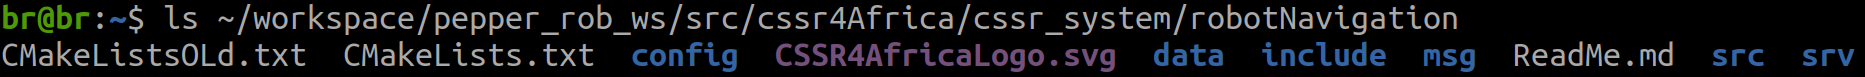
\includegraphics[width=\linewidth]{Images/navigation_folder.png}
    \caption{Screenshot of expected output showing the files and folders in the robotNavigation node from the executed command}
    \label{fig:sample robot navigation folder structure}
\end{figure}

\subsubsection*{Configure the Node}
The \verb|robotNavigation| node is configured using pre-defined map and setting files. The configuration parameters are set in the \verb|robotNavigationConfiguration.ini| listed in Table \ref{tab:robotNavigationConfiguration.ini}. If necessary, update the configuration values in the configuration file before starting the node.

\subsubsection*{Starting the Node}
\begin{notebox}
Ensure that the robot localization node is running. If not, execute the following command:
\begin{lstlisting}[style=withoutNumbering, language=bash]
rosrun cssr_system robotLocalization
\end{lstlisting}
\end{notebox}

\noindent To start the \verb|robotNavigation| Node, execute the following command:
\begin{lstlisting}[style=withoutNumbering, language=bash]
rosrun cssr_system robotNavigation
\end{lstlisting}
This will initialize the navigation system and display status messages indicating the node running.

\begin{figure}[H]
    \centering
    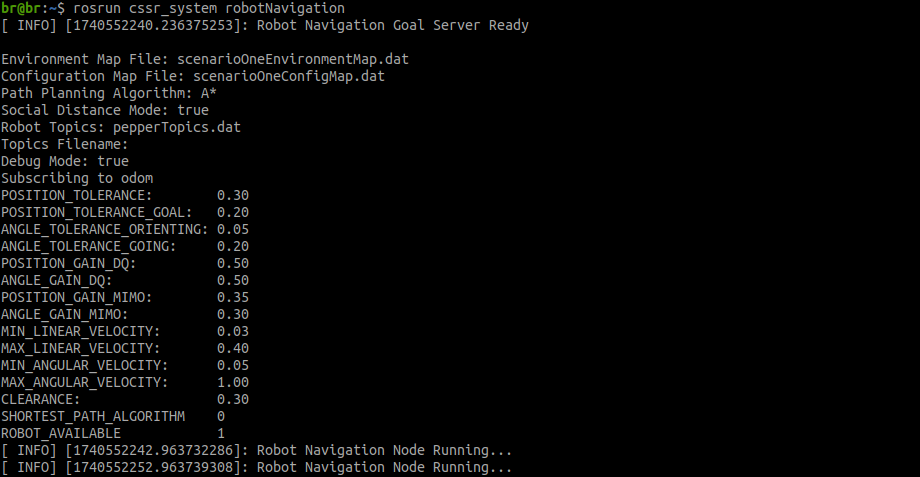
\includegraphics[width=\linewidth]{Images/rosrun_navigation.png}
    \caption{Screenshot of the output of running the robotNavigation node.}
    \label{fig:rosrun_navigation}
\end{figure}

\subsection{Interacting with the Node}
\noindent To check the robot's current pose, execute the following command.
\begin{lstlisting}[style=withoutNumbering, language=bash]
rostopic echo /robotNavigation/pose
\end{lstlisting}
\noindent This will output the robot’s current position and orientation.

\subsubsection*{Resetting the Pose}
To manually set the robot’s pose, use the following service call:
\begin{lstlisting}[style=withoutNumbering, language=bash]
rosservice call /robotLocalization/set_pose <x_position> <y_position> <theta>
\end{lstlisting}
\begin{figure}[H]
    \centering
    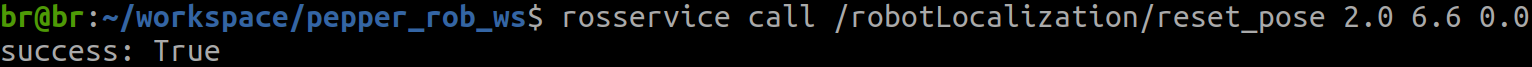
\includegraphics[width=\linewidth]{Images/reset_pose.png}
    \caption{Screenshot of the rosservice call to set the position responds a success message of true.}
    \label{fig:reset_pose}
\end{figure}
\subsubsection*{Sending a Goal}
To command the robot to navigate to a specific position, use:
\begin{lstlisting}[style=withoutNumbering, language=bash]
rosservice call /robotNavigation/set_goal goal_x goal_y goal_theta
\end{lstlisting}
\begin{lstlisting}[style=withoutNumbering, language=bash]
Example:
rosservice call /robotNavigation/set_goal 2.0 6.6 0.0
\end{lstlisting}
If the navigation is successful, a confirmation message will be displayed.
\begin{figure}[H]
    \centering
    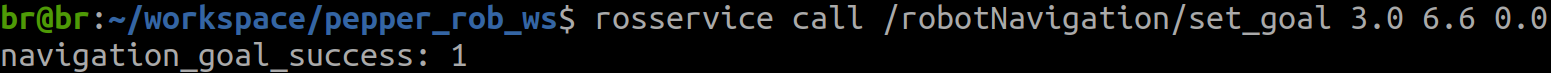
\includegraphics[width=\linewidth]{Images/set_goal.png}
    \caption{Screenshot of the rosservice call to set goal for navigation responds a success message of 1.}
    \label{fig:set_goal}
\end{figure}

\newpage
\section{Unit Test}
%===============================================================
Testing is a crucial step in the software development lifecycle, ensuring that each component of the system performs as expected. The \verb|robotNavigation| node requires validation to confirm that path planning, goal execution, and obstacle avoidance work reliably under various conditions. Unit testing is employed to assess these functionalities independently, following the structured testing guidelines outlined in \href{https://cssr4africa.github.io/deliverables/CSSR4Africa_Deliverable_D3.5.pdf}{Deliverable D3.5}, System Integration and Quality Assurance.
The \verb|robotNavigation| node comprises several key operations, including path planning, waypoint generation, pose retrieval, and velocity command execution. To ensure that these components function correctly, a unit test is developed using the GoogleTest framework. These tests isolate functions and verify their expected behavior under different scenarios.

\subsection{File Organization and Its Purposes}
\vspace*{0.5em}
\begin{figure}[H]
	\renewcommand*\DTstyle{\ttfamily}
	\dirtree{%
		.1 unit\_tests.
		.2 robotNavigationTest.
		.3 config.
		.4 robotNavigationTestConfiguration.ini.
		.3 data.
		.4 astarAlgorithmInput.dat.
		.4 bfsAlgorithmInput.dat.
		.4 boundaryTestInput.dat.
		.4 dijkstraAlgorithmInput.dat.
		.4 navigationServiceInput.dat.
		.4 pepperTopics.dat.
		.4 robotNavigationTestOutput.dat.
		.3 include.
		.4 robotNavigationTest.
		.5 robotNavigationTestInterface.h.
		.3 launch.
		.4 robotNavigationLaunchTestHarness.launch.
		.4 robotNavigationLaunchTestRobot.launch.
		.3 msg.
		.4 Goal.msg.
		.3 src.
		.4 robotNavigationDriver.cpp.
		.4 robotNavigationTestApplication.cpp.
		.4 robotNavigationTestImplementation.cpp.
		.3 srv.
		.4 setGoal.srv.
		.4 setPose.srv.
		.3 CSSR4AfricaLogo.svg.
		.3 CMakeLists.txt.
		.3 README.md.
		.2 CMakeLists.txt.
		.2 package.xml.
	}
	\caption{File structure of the robotNavigation unit test}
	\label{fig:navigation_test_structure}
\end{figure}

\noindent The \texttt{robotNavigationTest} folder is structured to support unit testing of the Robot Navigation unit test Node. The \texttt{src} directory contains \texttt{robotNavigationDriver.cpp}, which serves as the driver for test execution, \texttt{robotNavigationTestApplication.cpp}, which manages the test flow, and \texttt{robotNavigationTestImplementation.cpp}, which provides the core test logic.\\


\noindent The \texttt{config} directory houses the \texttt{robotNavigationTestConfiguration.ini} file, which defines test parameters such as goal positions and navigation constraints, allowing customization of test cases. The \texttt{data} folder contains \texttt{navigationServiceInput.dat}, \texttt{astarAlgorithmInput.dat}, \texttt{bfsAlgorithmInput.dat}, \texttt{boundaryTestInput.dat}, \texttt{dijkstraAlgorithmInput.dat} which stores predefined navigation goals for the tests, and \texttt{navigationUnitTestLogs.log}, which captures the test execution logs, recording timestamps and goal completion statuses for debugging and validation.



\subsection{Test Environment Setup}
Before executing the robot navigation units tests, the testing environment must be properly configured.

\begin{enumerate}
\item Install all necessary dependencies:
\begin{lstlisting}[style=withoutNumbering, language=bash]
cd ~/workspace/pepper_rob_ws
rosdep install --from-paths src --ignore-src -r -y
\end{lstlisting}

\item Clone the CSSR4Africa repository into the workspace (if not already cloned):
\begin{lstlisting}[style=withoutNumbering, language=bash]
cd ~/workspace/pepper_rob_ws/src
\end{lstlisting}
\begin{lstlisting}[style=withoutNumbering, language=bash]
git clone https://github.com/cssr4africa/cssr4africa.git
\end{lstlisting}
\item Build the workspace and source the environment:
\begin{lstlisting}[style=withoutNumbering, language=bash]
cd ~/workspace/pepper_rob_ws
\end{lstlisting}

\begin{lstlisting}[style=withoutNumbering, language=bash]
catkin_make
\end{lstlisting}

\begin{lstlisting}[style=withoutNumbering, language=bash]
source devel/setup.bash
\end{lstlisting}
\end{enumerate}

\noindent The test execution is controlled using the configuration file \texttt{robotNavigationTestConfiguration.ini}, located in the \texttt{config} directory of the unit test package. This file defines the test parameters, including position tolerance, angle tolerance, and social distance.

\subsection{Test Cases}
The test cases evaluate the ability of the \texttt{robotNavigation} node to process navigation requests and reach predefined goals.

\begin{enumerate}
    \item SetGoalServiceAvailable: Verifies that the \texttt{/robotNavigation/set\_goal} service is available before sending navigation commands.
    \item SendNavigationGoalFromFile: Reads a list of predefined goals from the \texttt{test\_goals.dat} file and sends them sequentially. The robot's response is validated against expected success values.
\end{enumerate}

\subsection{Executing the Robot Navigation Unit Test}
To start the unit test, use the following command:

\begin{lstlisting}[style=withoutNumbering, language=bash]
cd ~/workspace/pepper_rob_ws
\end{lstlisting}
\begin{lstlisting}[style=withoutNumbering, language=bash]
rosrun unit_tests robotNavigationTest
\end{lstlisting}
Upon execution, the test sequence is initiated, and results are logged in the \texttt{navigationUnitTestLogs.log} file.
\begin{figure}[H]
    \centering
    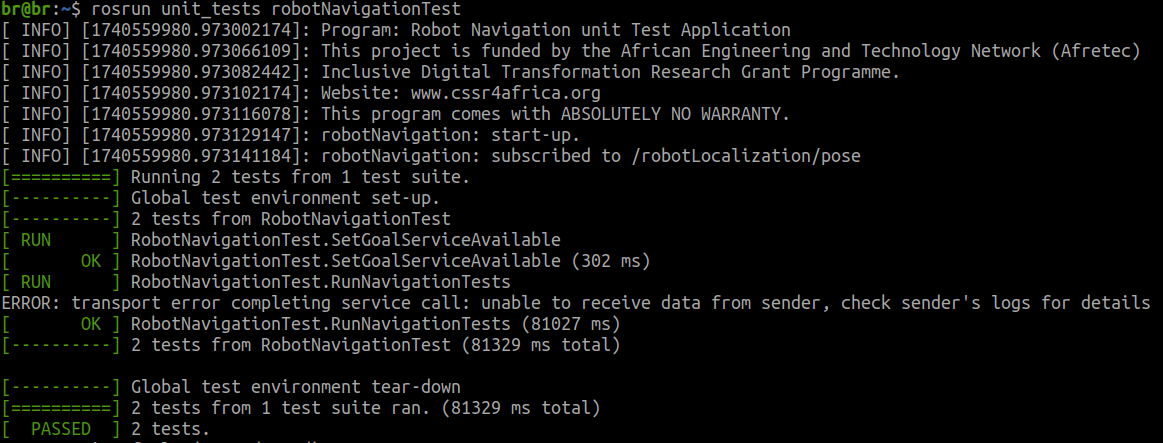
\includegraphics[width=\linewidth]{Images/unit-test-terminal.png}
    \caption{Screenshot of the unit test command running.}
    \label{fig:unit_test_terminal}
\end{figure}

\subsection{Test Results}
The results of the unit tests are categorized based on success and failure conditions. If a test case passes, the corresponding success message is logged. Otherwise, an error message is generated with relevant debugging details. The test reports are attached in Appendix I.

\newpage
\appendix

\begin{landscape} 
\section*{Appendix I: Unit Test Logs}
\addcontentsline{toc}{section}{Appendix I: Unit Test Logs}

\small  
\begin{verbatim}
[2025-02-26 10:08:10] =======================================================================
[2025-02-26 10:08:10] === New Robot Navigation Test Run Started at 2025-02-26 10:08:10 ===
[2025-02-26 10:08:10] =======================================================================
[2025-02-26 10:08:10] Initializing Robot Navigation Node: PASSED
[2025-02-26 10:08:10] -----------------------------------------------------------------------
[2025-02-26 10:08:10] Test Case 1: Goal to (5.0, 6.6, 0.0)
[2025-02-26 10:08:10] Sending goal...
[2025-02-26 10:08:31] [SUCCESS] Goal reached: (5.000000, 6.600000, 0.000000)
[2025-02-26 10:08:31] Goal execution successful: PASSED
[2025-02-26 10:08:31] -----------------------------------------------------------------------
[2025-02-26 10:08:31] Test Case 2: Goal to (5.0, 2.0, 270.0)
[2025-02-26 10:08:31] Sending goal...
[2025-02-26 10:09:03] [SUCCESS] Goal reached: (5.000000, 2.000000, 270.000000)
[2025-02-26 10:09:03] Goal execution successful: PASSED
[2025-02-26 10:09:03] -----------------------------------------------------------------------
[2025-02-26 10:09:03] Test Case 3: Goal to (5.0, 6.6, 90.0)
[2025-02-26 10:09:03] Sending goal...
[2025-02-26 10:09:53] [SUCCESS] Goal reached: (5.000000, 6.600000, 90.000000)
[2025-02-26 10:09:53] Goal execution successful: PASSED
[2025-02-26 10:09:53] -----------------------------------------------------------------------
[2025-02-26 10:09:53] Test Case 4: Goal to (2.0, 6.6, 0.0)
[2025-02-26 10:09:53] Sending goal...
[2025-02-26 10:10:19] [SUCCESS] Goal reached: (2.000000, 6.600000, 0.000000)
[2025-02-26 10:10:19] Goal execution successful: PASSED
[2025-02-26 10:10:19] -----------------------------------------------------------------------
[2025-02-26 10:10:19] =======================================================================
[2025-02-26 10:10:19] === Robot Navigation Test Run Completed at 2025-02-26 10:10:19 ===
[2025-02-26 10:10:19] =======================================================================

[2025-02-26 10:53:01] =======================================================================
[2025-02-26 10:53:01] === New Robot Navigation Test Run Started at 2025-02-26 10:53:01 ===
[2025-02-26 10:53:01] =======================================================================
[2025-02-26 10:53:01] Initializing Robot Navigation Node: PASSED
[2025-02-26 10:53:01] -----------------------------------------------------------------------
[2025-02-26 10:53:01] Test Case 1: Goal to (3.2, 6.6, 0.0)
[2025-02-26 10:53:01] Sending goal...
[2025-02-26 10:53:10] [SUCCESS] Goal reached: (3.200000, 6.600000, 0.000000)
[2025-02-26 10:53:10] Goal execution successful: PASSED
[2025-02-26 10:53:10] -----------------------------------------------------------------------
[2025-02-26 10:53:10] Test Case 2: Goal to (3.2, 6.0, 270.0)
[2025-02-26 10:53:10] Sending goal...
[2025-02-26 10:53:11] [SUCCESS] Goal reached: (3.200000, 6.000000, 270.000000)
[2025-02-26 10:53:11] Goal execution successful: PASSED
[2025-02-26 10:53:11] -----------------------------------------------------------------------
[2025-02-26 10:53:11] Test Case 3: Goal to (2.0, 6.0, 180.0)
[2025-02-26 10:53:11] Sending goal...
[2025-02-26 10:53:28] [SUCCESS] Goal reached: (2.000000, 6.000000, 180.000000)
[2025-02-26 10:53:28] Goal execution successful: PASSED
[2025-02-26 10:53:28] -----------------------------------------------------------------------
[2025-02-26 10:53:28] Test Case 4: Goal to (2.0, 6.6, 0.0)
[2025-02-26 10:53:28] Sending goal...
[2025-02-26 10:54:22] [SUCCESS] Goal reached: (2.000000, 6.600000, 0.000000)
[2025-02-26 10:54:22] Goal execution successful: PASSED
[2025-02-26 10:54:22] -----------------------------------------------------------------------
[2025-02-26 10:54:22] =======================================================================
[2025-02-26 10:54:22] === Robot Navigation Test Run Completed at 2025-02-26 10:54:22 ===
[2025-02-26 10:54:22] =======================================================================
\end{verbatim}
\end{landscape}  



\clearpage


\newpage
\bibliographystyle{unsrt}
%================================================================
\bibliography{cssr4africa.bib} 
\addcontentsline{toc}{section}{References}

\pagebreak
\section*{Principal Contributors}
%===============================================================
\label{contributors}
\addcontentsline{toc}{section}{Principal Contributors}
The main authors of this deliverable are as follows:
\blank
Birhanu Shimelis Girma, Carnegie Mellon University Africa.

\newpage
\section*{Document History}
%================================================================
\addcontentsline{toc}{section}{Document History}
\label{document_history}

\begin{description}
	
	\item [Version 1.0]~\\
	First draft. \\
	Birhanu Shimelis Girma. \\
	26 February 2025.
	
	\item [Version 1.1]~\\
	Added hyperlinks to all referenced deliverables for improved accessibility. \\
	Enhanced the Module Specification section with detailed descriptions of the three path planning algorithms (BFS, Dijkstra, and A*), including pseudocode. \\
	Standardized paragraph formatting throughout the document for better readability. \\
	Added a navigation process flowchart to visualize the complete workflow. \\
	Added proper captions and labels to file structure diagrams. \\
	Birhanu Shimelis Girma. \\
	18 April 2025.
		
	\item [Version 1.2]~\\
	Updated the file organization diagram. \\
	Updated Table \ref{tab:robotNavigationConfiguration.ini} to include robotType, environmentMap, and configurationSpaceMap parameters.\\
	Changed service name from reset\_pose to set\_pose in the body of document. \\
	Updated the commands as well following the change in service name and updated it in the body. \\
	Birhanu Shimelis Girma. \\
	18 April 2025.

\end{description}

\end{document}
